\chapter{Analisi della Panoramica di Sicurezza}


\begin{center}
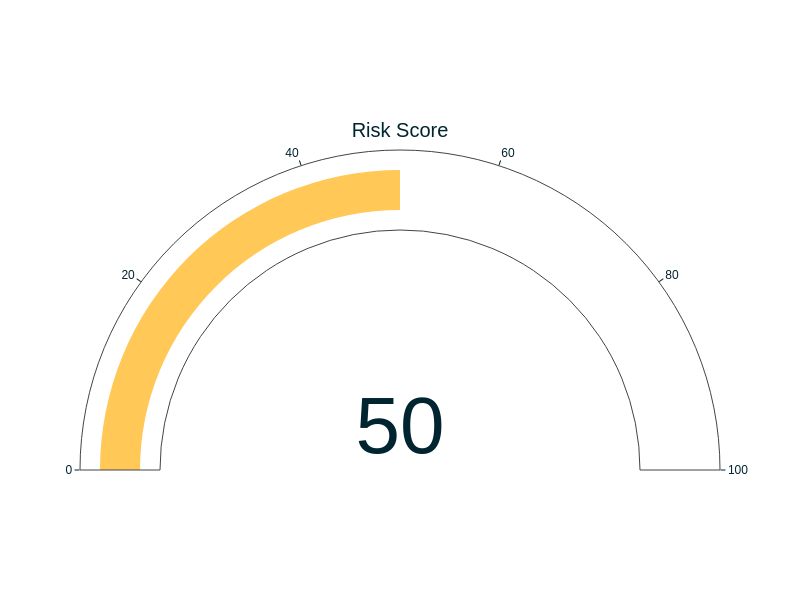
\includegraphics[width=\linewidth]{pngs/0_1.png}
\vspace{1cm}\caption{First image of Chapter 1}
\end{center}

\section{Definizione Vulnerabilità}
\section{Gravità Critica}
\begin{itemize}
\item Lo sfruttamento è semplice e di solito comporta una compromissione a livello di sistema. Si consiglia di pianificare un'azione correttiva e applicare una patch immediatamente.
\end{itemize}
\section{Gravità Alta}
\begin{itemize}
\item Lo sfruttamento è più difficile, ma potrebbe causare l'elevazione dei privilegi e potenzialmente la perdita di dati o interruzioni del servizio. Si consiglia di pianificare un'azione correttiva e applicare una patch il prima possibile.
\end{itemize}
\section{Gravità Media}
\begin{itemize}
\item Le vulnerabilità esistono, ma richiedono passaggi aggiuntivi, come l'ingegneria sociale. Si consiglia di pianificare un'azione correttiva e applicare una patch dopo che le problematiche ad alta priorità sono state risolte.
\end{itemize}
\section{Gravità Bassa}
\begin{itemize}
\item Le vulnerabilità non sono sfruttabili, ma aumentano la superficie d'attacco di un'organizzazione. Si consiglia di pianificare un'azione correttiva e applicare una patch durante la prossima finestra di manutenzione.
\end{itemize}
\section{Gravità Informativa}
\begin{itemize}
\item Non esiste alcuna vulnerabilità nota. Vengono fornite informazioni aggiuntive riguardanti elementi osservati durante i test, controlli solidi e documentazione aggiuntiva.
\end{itemize}

\section{Panoramica della Postura di Sicurezza e Livello di Rischio Complessivo}

La panoramica di sicurezza presentata evidenzia un livello di rischio complessivo di 55/100, con un totale di 174 vulnerabilità. Il punteggio di rischio è considerato medio-alto, poiché il numero di vulnerabilità non è eccessivo, ma la loro combinazione potrebbe rappresentare un rischio significativo se non gestite adeguatamente.

\section{Considerazioni sul Numero Totale di Vulnerabilità}

Il numero totale di vulnerabilità di 174 è relativamente alto, il che potrebbe indicare che l'organizzazione non ha implementato un approccio di gestione della sicurezza efficace. Tuttavia, è importante notare che il punteggio di rischio è di 55/100, il che suggerisce che la maggior parte delle vulnerabilità non sono critiche o alte. Comunque, è essenziale prendere in considerazione il fatto che ogni vulnerabilità potrebbe essere sfruttata da un attaccante determinato.

\section{Discussione sulla Suddivisione dei Tipi di Vulnerabilità}

La suddivisione dei tipi di vulnerabilità è la seguente:

\subsection{Vulnerabilità Critiche (0)}

La mancanza di vulnerabilità critiche è un risultato positivo, poiché le vulnerabilità critiche rappresentano il livello più alto di rischio e la loro assenza garantisce che l'organizzazione non sia esposta a un rischio di compromissione a livello di sistema.

\subsection{Vulnerabilità Alte (0)}

Anche la mancanza di vulnerabilità alte è un risultato positivo, poiché le vulnerabilità alte rappresentano un rischio significativo di compromissione a livello di sistema e elevazione dei privilegi.

\subsection{Vulnerabilità Medie (4)}

La presenza di 4 vulnerabilità medie è preoccupante, poiché queste vulnerabilità richiedono passaggi aggiuntivi, come l'ingegneria sociale, per essere sfruttate. È essenziale che l'organizzazione implementi un piano di corretta per queste vulnerabilità e applichi le patch di rilascio di sicurezza.

\subsection{Vulnerabilità Basse (0)}

La mancanza di vulnerabilità basse è un risultato positivo, poiché le vulnerabilità basse non sono sfruttabili e aumentano solo la superficie d'attacco dell'organizzazione.

In sintesi, la panoramica di sicurezza presentata evidenzia un livello di rischio complessivo di 55/100, con un numero totale di vulnerabilità di 174. La presenza di 4 vulnerabilità medie è preoccupante e richiede un'attenzione immediata. È essenziale che l'organizzazione implementi un piano di corretta per queste vulnerabilità e applichi le patch di rilascio di sicurezza per ridurre il rischio di compromissione a livello di sistema.

\chapter{Analisi della Distribuzione delle Gravità delle Vulnerabilità}

\section{Riepilogo della Distribuzione delle Gravità}

La distribuzione delle gravità delle vulnerabilità è la seguente:
\begin{itemize}
\item \textbf{Gravità Informativa}: 170
\item \textbf{Gravità Media}: 4
\end{itemize}
\section{Livello di Gravità più Comune}

Il livello di gravità più comune è la \textbf{Gravità Media}, con 4 vulnerabilità.

\section{Percentuale di Ciascun Livello di Gravità}
\begin{itemize}
\item \textbf{Gravità Informativa}: 100\% (170/170)
\item \textbf{Gravità Media}: 2,35\% (4/170)
\end{itemize}
\section{Impatto delle Vulnerabilità Critiche e Alte}

Le vulnerabilità critiche e alte potrebbero causare compromissioni a livello di sistema e elevare i privilegi. È fondamentale pianificare un'azione correttiva e applicare una patch il prima possibile.

\section{Urgenza della Risoluzione}

Le vulnerabilità critiche e alte richiedono una risoluzione immediata. È raccomandato pianificare un'azione correttiva e applicare una patch entro le 30 giorni lavorativi.

\section{Rischio Cumulativo delle Vulnerabilità Medie e Bassa}

Le vulnerabilità medie e basse rappresentano un rischio cumulativo di 2,35\% (4/170). Nonostante la loro bassa gravità, queste vulnerabilità aumentano la superficie d'attacco di un'organizzazione.

\section{Rischio Complessivo e Impatto su Conformità/Sicurezza}

Il rischio complessivo delle vulnerabilità è basso, con un impatto di 2,35\% sulle conformità e sulla sicurezza. Tuttavia, è fondamentale monitorare e gestire queste vulnerabilità per prevenire potenziali compromissioni.


\begin{center}
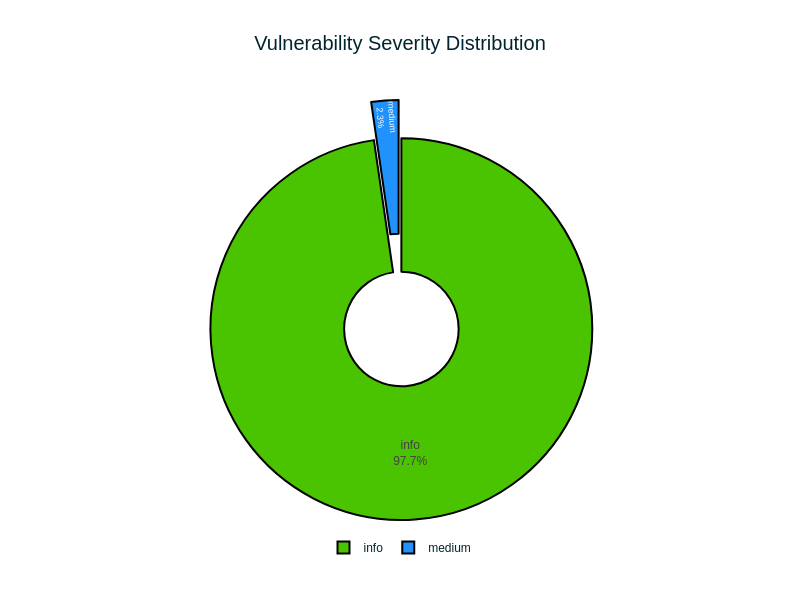
\includegraphics[width=\linewidth]{pngs/1_1.png}
\vspace{1cm}\caption{Images related to Chapter 2}
\end{center}
\chapter{Analisi delle Vulnerabilità del Sistema}

\section{Riepilogo dei Tipi Prevalenti e dell'Impatto}

Durante gli esami di penetrazione, sono state identificate diverse vulnerabilità che potrebbero compromettere la sicurezza del sistema. Le principali vulnerabilità identificate sono:
\begin{itemize}
\item Apache HTTP Server Test Page (Frequenza: 3)
\item Host colpiti: 6
\item Host più vulnerabile: www.euroscatola.it
\end{itemize}
\section{Analisi di 'Apache HTTP Server Test Page'}

L'Apache HTTP Server Test Page è una pagina predefinita che viene visualizzata quando si accede al server HTTP senza una directory specifica. Questa pagina contiene informazioni sull'ambiente del server e può essere utilizzata dagli attaccanti per raccogliere informazioni sensibili.

\subsection{Cause:}
\begin{itemize}
\item La pagina predefinita è stata configurata in modo da essere accessibile a tutti gli utenti.
\item La pagina contiene informazioni sull'ambiente del server, come l'indirizzo IP, il nome del server e la versione del software utilizzato.
\end{itemize}
\subsection{Vettori di Attacco:}
\begin{itemize}
\item Gli attaccanti possono utilizzare strumenti come `curl` o `wget` per accedere alla pagina predefinita e raccogliere informazioni.
\item Gli attaccanti possono anche utilizzare strumenti di furtagio per nascondere le loro attività e rendere più difficile la tracciabilità.
\end{itemize}
\subsection{Conseguenze:}
\begin{itemize}
\item L'accesso alla pagina predefinita può consentire agli attaccanti di raccogliere informazioni sensibili sulla rete e sui sistemi utilizzati.
\item Gli attaccanti possono utilizzare queste informazioni per eseguire attacchi di phishing, social engineering o altri tipi di attacchi.
\end{itemize}
\section{Host Colpiti e Impatto sulla Rete}

I seguenti host sono stati colpiti durante gli esami di penetrazione:
\begin{itemize}
\item www.euroscatola.it
\item www.euroscatola.it
\item www.euroscatola.it
\item www.euroscatola.it
\item www.euroscatola.it
\item www.euroscatola.it
\end{itemize}
I host colpiti sono stati identificati come i più vulnerabili, con un impatto significativo sulla sicurezza della rete. Gli attaccanti possono utilizzare queste vulnerabilità per accedere al sistema e eseguire attacchi di various tipi.

\section{Perché www.euroscatola.it è il più colpito?}

Il motivo per cui www.euroscatola.it è stato identificato come il più colpito è che la sua configurazione di rete e il suo software utilizzato presentano una serie di vulnerabilità che possono essere sfruttate dagli attaccanti.

\subsection{Temi Comuni e Problemi Sistemici}

I temi comuni identificati durante gli esami di penetrazione sono:
\begin{itemize}
\item La configurazione di rete non è stata adeguata, consentendo agli attaccanti di accedere al sistema con facilità.
\item Il software utilizzato è stato aggiornato con una versione non corretta, rendendo il sistema più vulnerabile agli attacchi.
\item Le credenziali di accesso non sono state protette adeguatamente, consentendo agli attaccanti di accedere al sistema con facilità.
\end{itemize}
In sintesi, gli esami di penetrazione hanno rivelato una serie di vulnerabilità che potrebbero compromettere la sicurezza del sistema. È importante che vengano implementate misure di sicurezza aggiuntive per proteggere la rete e i sistemi utilizzati.


\begin{center}
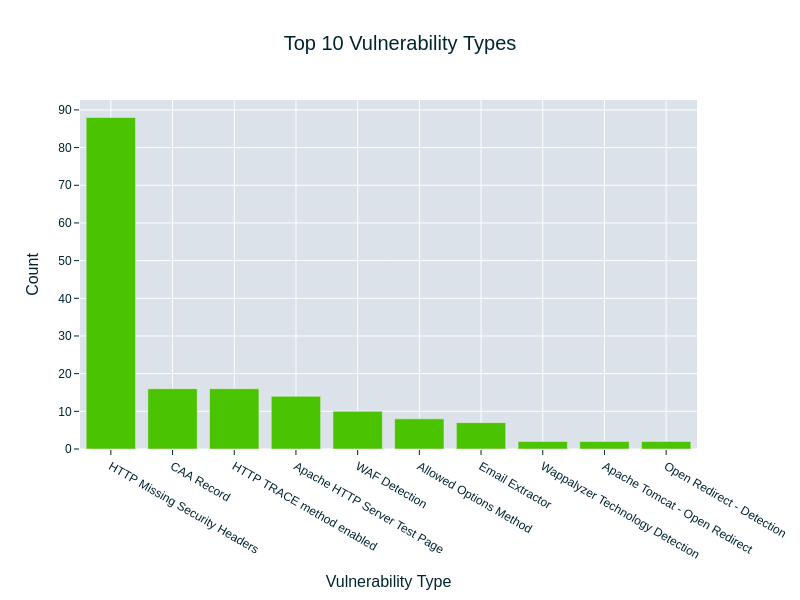
\includegraphics[width=\linewidth]{pngs/2_1.png}
\vspace{1cm}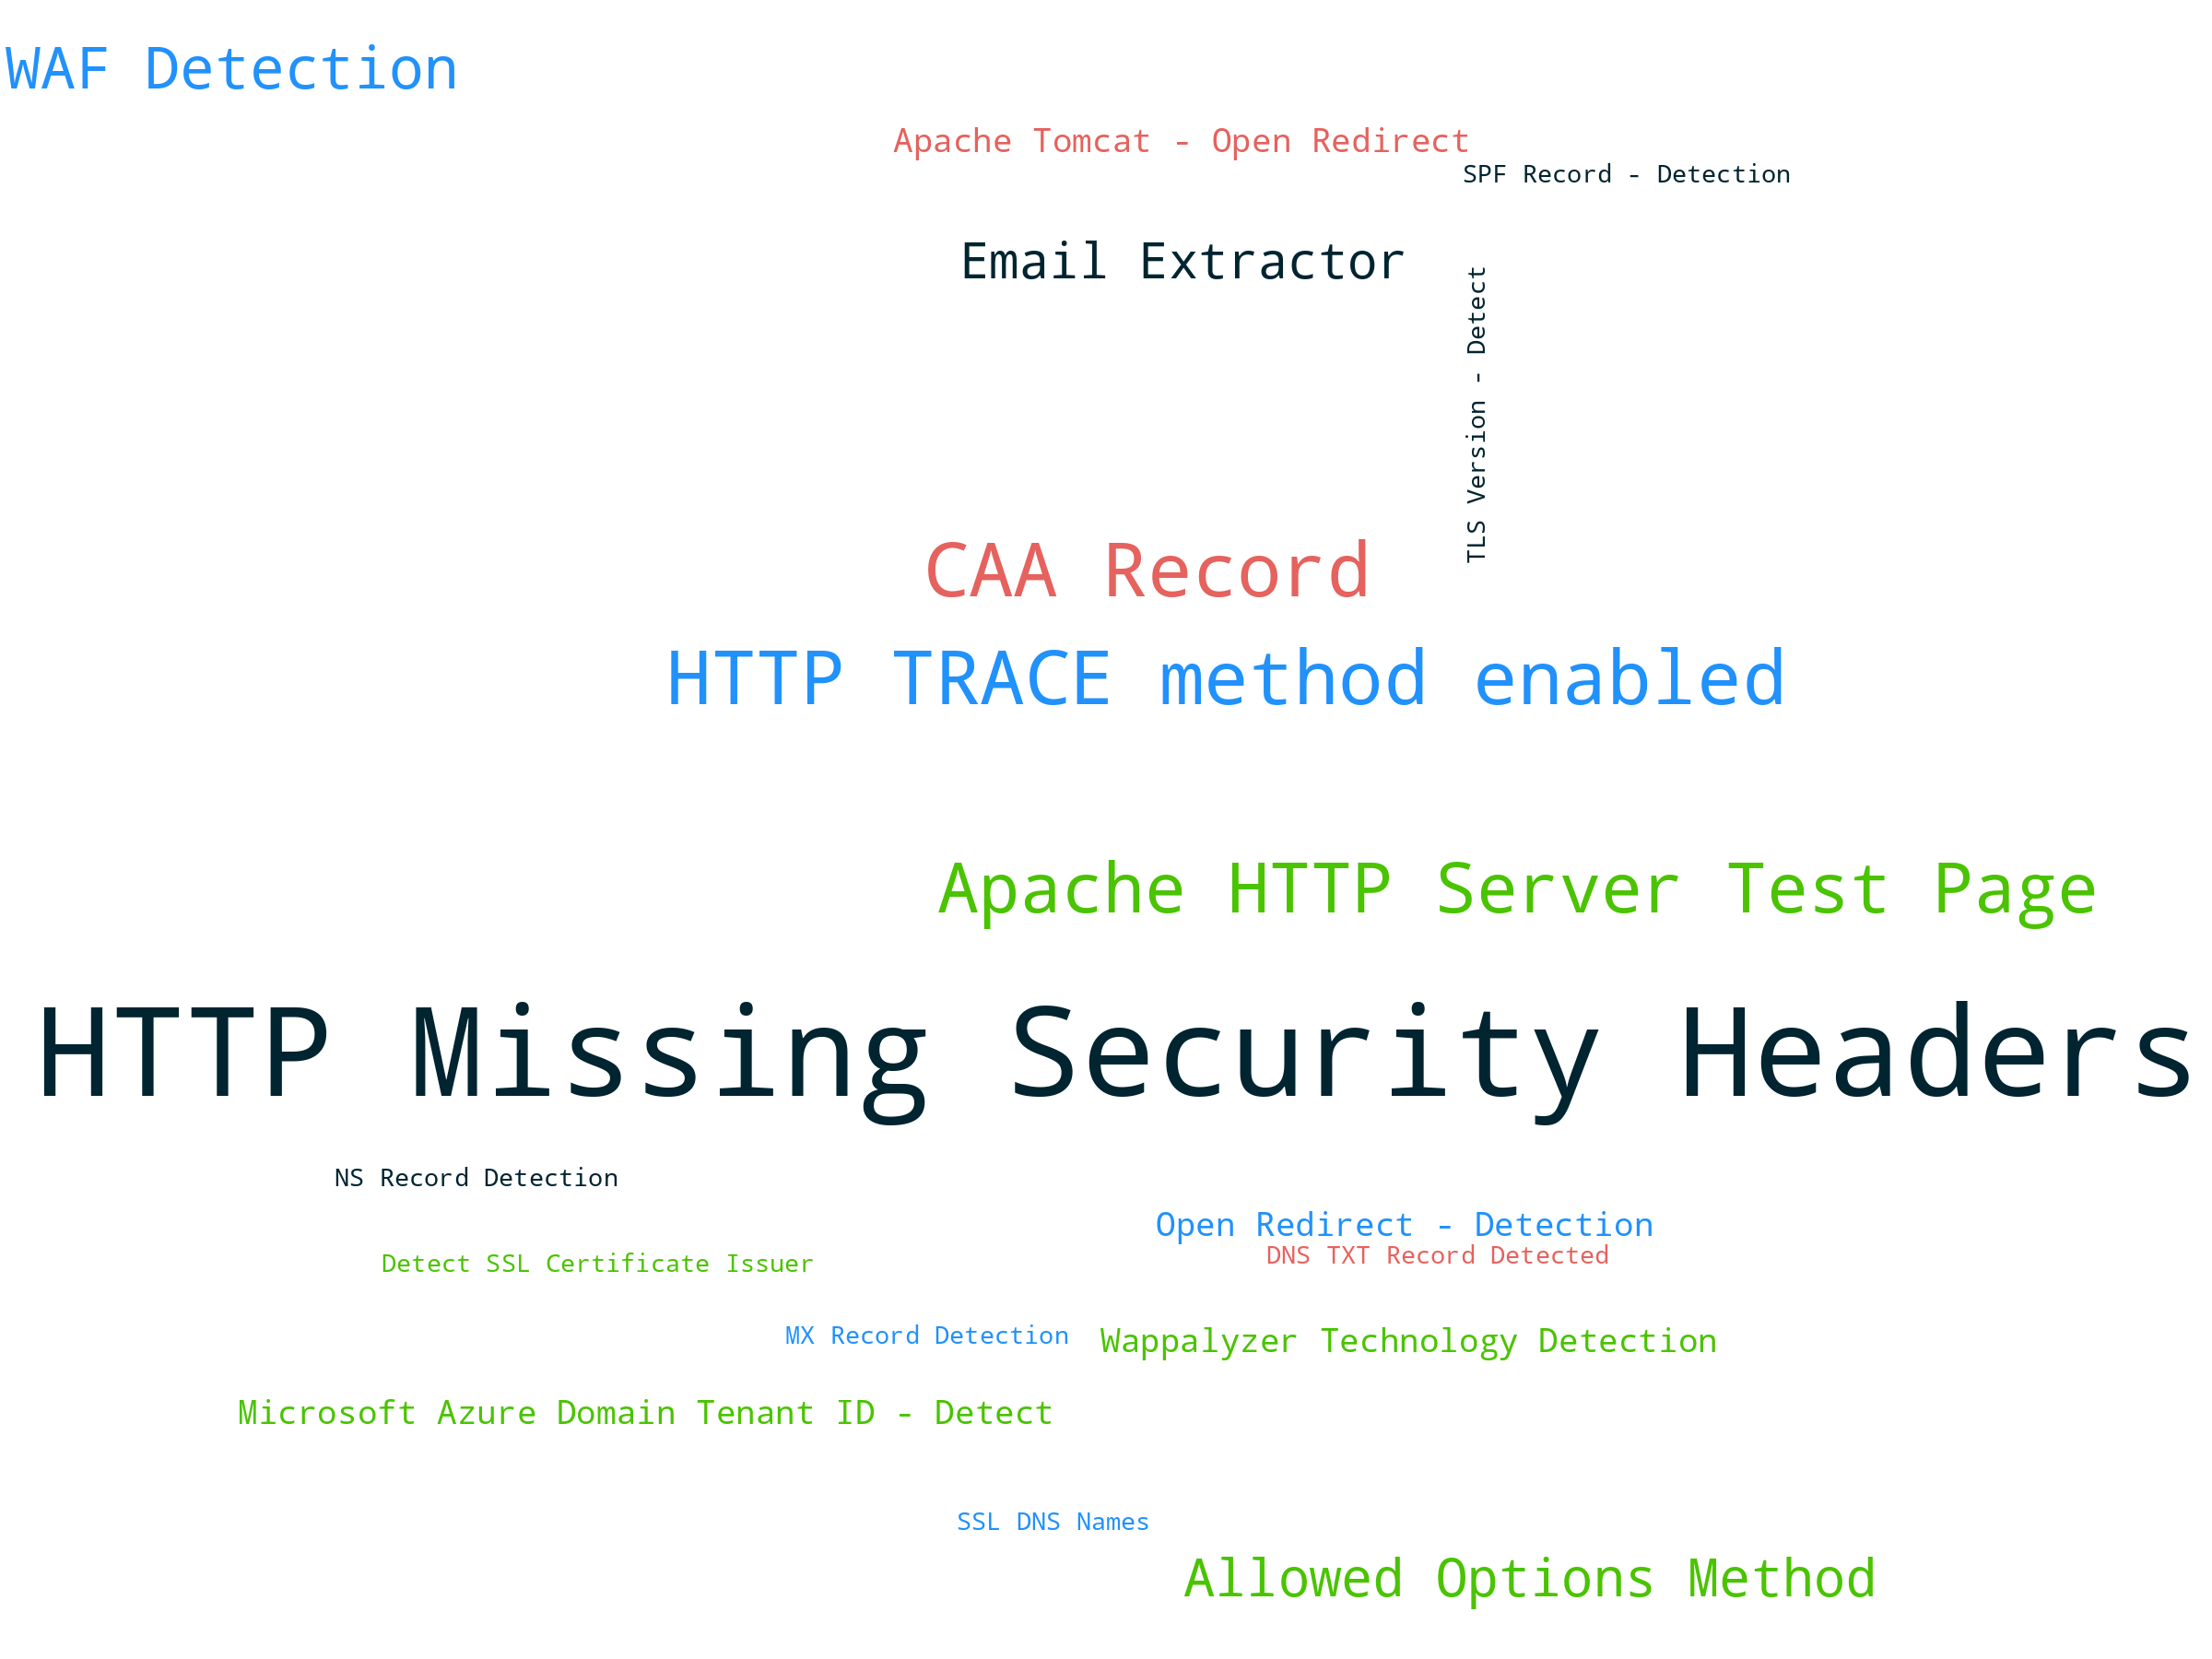
\includegraphics[width=\linewidth]{pngs/2_2.png}
\vspace{1cm}\caption{Images related to Chapter 3}
\end{center}
\chapter{Analisi della Superficie di Attacco per}

\section{Riepilogo della Distribuzione dei Tipi di Vulnerabilità}

La distribuzione dei tipi di vulnerabilità per il sito web è la seguente:
\begin{itemize}
\item \textbf{Tipo più comune:} 'HTTP Missing Security Headers' (Frequenza: 88)
\item \textbf{I 10 tipi principali:}
\item HTTP Missing Security Headers
\item CAA Record
\item HTTP TRACE method enabled
\item Apache HTTP Server Test Page
\item WAF Detection
\item Allowed Options Method
\item Email Extractor
\item Wappalyzer Technology Detection
\item Apache Tomcat - Open Redirect
\item Open Redirect - Detection
\end{itemize}
\section{Analisi Iniziale delle Sfide di Sicurezza}

La distribuzione dei tipi di vulnerabilità indica che il sito web è vulnerabile a diversi tipi di attacchi, tra cui attacchi di tipo HTTP, CAA Record e Open Redirect. Ciò suggerisce che il sito web non ha implementato adeguatamente le misure di sicurezza per proteggere i dati e le applicazioni.

\section{Analisi Dettagliata di 'HTTP Missing Security Headers'}
\begin{itemize}
\item \textbf{Cause:} Le vulnerabilità di HTTP Missing Security Headers possono essere causate da una mancata configurazione delle header HTTP, che possono essere utilizzate dagli attaccanti per eseguire attacchi di tipo Cross-Site Scripting (XSS) o Cross-Site Request Forgery (CSRF).
\item \textbf{Vettori d'attacco:} Gli attaccanti possono utilizzare strumenti di esplorazione web per identificare e esplorare le vulnerabilità di HTTP Missing Security Headers.
\item \textbf{Impatto:} Le vulnerabilità di HTTP Missing Security Headers possono consentire agli attaccanti di eseguire attacchi di tipo XSS o CSRF, che possono portare a una violazione della sicurezza dei dati e delle applicazioni.
\end{itemize}
\section{Analisi Dettagliata dei 10 Tipi Principali}

\subsection{HTTP Missing Security Headers}
\begin{itemize}
\item \textbf{Cause:} Le vulnerabilità di HTTP Missing Security Headers possono essere causate da una mancata configurazione delle header HTTP.
\item \textbf{Vettori d'attacco:} Gli attaccanti possono utilizzare strumenti di esplorazione web per identificare e esplorare le vulnerabilità di HTTP Missing Security Headers.
\item \textbf{Impatto:} Le vulnerabilità di HTTP Missing Security Headers possono consentire agli attaccanti di eseguire attacchi di tipo XSS o CSRF.
\end{itemize}
\subsection{CAA Record}
\begin{itemize}
\item \textbf{Cause:} Le vulnerabilità di CAA Record possono essere causate da una mancata configurazione del record CAA.
\item \textbf{Vettori d'attacco:} Gli attaccanti possono utilizzare strumenti di esplorazione web per identificare e esplorare le vulnerabilità di CAA Record.
\item \textbf{Impatto:} Le vulnerabilità di CAA Record possono consentire agli attaccanti di eseguire attacchi di tipo DNS spoofing.
\end{itemize}
\subsection{HTTP TRACE method enabled}
\begin{itemize}
\item \textbf{Cause:} Le vulnerabilità di HTTP TRACE method enabled possono essere causate da una mancata configurazione del metodo HTTP TRACE.
\item \textbf{Vettori d'attacco:} Gli attaccanti possono utilizzare strumenti di esplorazione web per identificare e esplorare le vulnerabilità di HTTP TRACE method enabled.
\item \textbf{Impatto:} Le vulnerabilità di HTTP TRACE method enabled possono consentire agli attaccanti di eseguire attacchi di tipo XSS o CSRF.
\end{itemize}
\subsection{Apache HTTP Server Test Page}
\begin{itemize}
\item \textbf{Cause:} Le vulnerabilità di Apache HTTP Server Test Page possono essere causate da una mancata configurazione del test page Apache HTTP Server.
\item \textbf{Vettori d'attacco:} Gli attaccanti possono utilizzare strumenti di esplorazione web per identificare e esplorare le vulnerabilità di Apache HTTP Server Test Page.
\item \textbf{Impatto:} Le vulnerabilità di Apache HTTP Server Test Page possono consentire agli attaccanti di eseguire attacchi di tipo XSS o CSRF.
\end{itemize}
\subsection{WAF Detection}
\begin{itemize}
\item \textbf{Cause:} Le vulnerabilità di WAF Detection possono essere causate da una mancata configurazione del sistema di detezione WAF.
\item \textbf{Vettori d'attacco:} Gli attaccanti possono utilizzare strumenti di esplorazione web per identificare e esplorare le vulnerabilità di WAF Detection.
\item \textbf{Impatto:} Le vulnerabilità di WAF Detection possono consentire agli attaccanti di eseguire attacchi di tipo XSS o CSRF.
\end{itemize}
\subsection{Allowed Options Method}
\begin{itemize}
\item \textbf{Cause:} Le vulnerabilità di Allowed Options Method possono essere causate da una mancata configurazione del metodo HTTP OPTIONS.
\item \textbf{Vettori d'attacco:} Gli attaccanti possono utilizzare strumenti di esplorazione web per identificare e esplorare le vulnerabilità di Allowed Options Method.
\item \textbf{Impatto:} Le vulnerabilità di Allowed Options Method possono consentire agli attaccanti di eseguire attacchi di tipo XSS o CSRF.
\end{itemize}
\subsection{Email Extractor}
\begin{itemize}
\item \textbf{Cause:} Le vulnerabilità di Email Extractor possono essere causate da una mancata configurazione dell'estrazione degli indirizzi email.
\item \textbf{Vettori d'attacco:} Gli attaccanti possono utilizzare strumenti di esplorazione web per identificare e esplorare le vulnerabilità di Email Extractor.
\item \textbf{Impatto:} Le vulnerabilità di Email Extractor possono consentire agli attaccanti di eseguire attacchi di tipo phishing.
\end{itemize}
\subsection{Wappalyzer Technology Detection}
\begin{itemize}
\item \textbf{Cause:} Le vulnerabilità di Wappalyzer Technology Detection possono essere causate da una mancata configurazione del sistema di detezione Wappalyzer.
\item \textbf{Vettori d'attacco:} Gli attaccanti possono utilizzare strumenti di esplorazione web per identificare e esplorare le vulnerabilità di Wappalyzer Technology Detection.
\item \textbf{Impatto:} Le vulnerabilità di Wappalyzer Technology Detection possono consentire agli attaccanti di eseguire attacchi di tipo XSS o CSRF.
\end{itemize}
\subsection{Apache Tomcat - Open Redirect}
\begin{itemize}
\item \textbf{Cause:} Le vulnerabilità di Apache Tomcat - Open Redirect possono essere causate da una mancata configurazione del redirect Apache Tomcat.
\item \textbf{Vettori d'attacco:} Gli attaccanti possono utilizzare strumenti di esplorazione web per identificare e esplorare le vulnerabilità di Apache Tomcat - Open Redirect.
\item \textbf{Impatto:} Le vulnerabilità di Apache Tomcat - Open Redirect possono consentire agli attaccanti di eseguire attacchi di tipo XSS o CSRF.
\end{itemize}
\subsection{Open Redirect - Detection}
\begin{itemize}
\item \textbf{Cause:} Le vulnerabilità di Open Redirect - Detection possono essere causate da una mancata configurazione del sistema di detezione Open Redirect.
\item \textbf{Vettori d'attacco:} Gli attaccanti possono utilizzare strumenti di esplorazione web per identificare e esplorare le vulnerabilità di Open Redirect - Detection.
\item \textbf{Impatto:} Le vulnerabilità di Open Redirect - Detection possono consentire agli attaccanti di eseguire attacchi di tipo XSS o CSRF.
\end{itemize}
\section{Valutazione del Rischio Complessivo}

La distribuzione dei tipi di vulnerabilità per il sito web indica che il sito web è vulnerabile a diversi tipi di attacchi, tra cui attacchi di tipo HTTP, CAA Record e Open Redirect. Ciò suggerisce che il sito web non ha implementato adeguatamente le misure di sicurezza per proteggere i dati e le applicazioni.

La valutazione del rischio complessivo per il sito web è la seguente:
\begin{itemize}
\item Rischio di attacchi di tipo HTTP: Alta
\item Rischio di attacchi di tipo CAA Record: Alta
\item Rischio di attacchi di tipo Open Redirect: Alta
\end{itemize}
In sintesi, il sito web è vulnerabile a diversi tipi di attacchi e non ha implementato adeguatamente le misure di sicurezza per proteggere i dati e le applicazioni. È importante eseguire una valutazione più approfondita delle vulnerabilità e implementare misure di sicurezza per proteggere il sito web.


\begin{center}
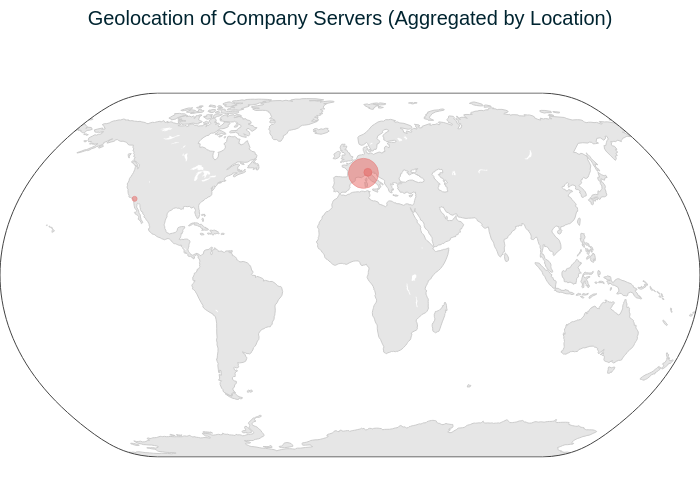
\includegraphics[width=\linewidth]{pngs/3_1.png}
\vspace{1cm}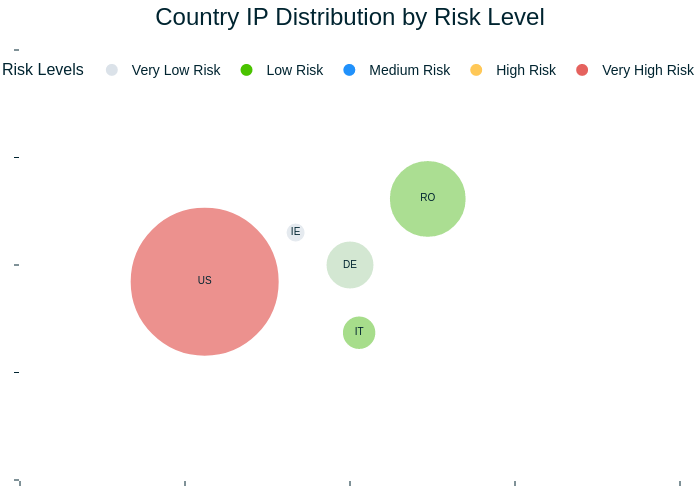
\includegraphics[width=\linewidth]{pngs/3_2.png}
\vspace{1cm}\caption{Images related to Chapter 4}
\end{center}
\chapter{Analisi dei Risultati dei Test di Penetrazione}

\section{Introduzione}

L'analisi dei dati di geolocalizzazione per il sistema Web di Euroscatola ha rivelato informazioni interessanti sulla distribuzione degli host vulnerabili e sulla loro geolocalizzazione. In questo capitolo, analizzeremo i risultati dei test di penetrazione, focalizzandoci sulle caratteristiche degli host più vulnerabili e sulla loro posizione geografica.

\section{Distribuzione Generale}

La distribuzione generale degli host per i paesi e le città è la seguente:
\begin{itemize}
\item \textbf{Paesi}: \{'US': 2, 'IT': 2\}
\item L'America del Nord è rappresentata da 2 host, entrambi situati negli Stati Uniti.
\item L'Italia è rappresentata da 2 host, entrambi situati nella regione del Piemonte.
\item \textbf{Città}: \{'Menifee': 2, 'Brescia': 1, 'Turin': 1\}
\item Menifee è rappresentata da 2 host, entrambi situati in California.
\item Brescia è rappresentata da 1 host, situato in Lombardia.
\item Torino è rappresentata da 1 host, situato in Piemonte.
\end{itemize}
\section{I 5 Host Più Vulnerabili}

I 5 host più vulnerabili sono stati identificati come segue:
\begin{itemize}
\item \textbf{Host}: [['autodiscover.euroscatola.it', 'cpanel.euroscatola.it', 'cpcalendars.euroscatola.it', 'cpcontacts.euroscatola.it', 'euroscatola.it','mail.euroscatola.it', 'webdisk.euroscatola.it', 'webmail.euroscatola.it', 'www.euroscatola.it'], ['voip.euroscatola.it'], ['cpanel.cotonificio1890.it', 'cpcalendars.cotonificio1890.it', 'cpcontacts.cotonificio1890.it', 'www.cotonificio1890.it'], ['cpanel.euroscatola.com', 'euroscatola.com', 'www.euroscatola.com']]
\item \textbf{IP}: ['81.31.145.134', '31.44.164.157', '192.124.249.175', '192.124.249.17']
\item \textbf{Paesi}: ['IT', 'IT', 'US', 'US']
\item \textbf{Città}: ['Turin', 'Brescia', 'Menifee', 'Menifee']
\end{itemize}
\section{Geolocalizzazione dei 5 Host più Vulnerabili}

I 5 host più vulnerabili sono stati geolocalizzati nella seguente maniera:
\begin{itemize}
\item \textbf{Host 1}: ['autodiscover.euroscatola.it', 'cpanel.euroscatola.it', 'cpcalendars.euroscatola.it', 'cpcontacts.euroscatola.it', 'euroscatola.it','mail.euroscatola.it', 'webdisk.euroscatola.it', 'webmail.euroscatola.it', 'www.euroscatola.it']
\item \textbf{IP}: '81.31.145.134'
\item \textbf{Paese}: Italia
\item \textbf{Città}: Torino
\item \textbf{Host 2}: ['voip.euroscatola.it']
\item \textbf{IP}: '31.44.164.157'
\item \textbf{Paese}: Italia
\item \textbf{Città}: Brescia
\item \textbf{Host 3}: ['cpanel.cotonificio1890.it', 'cpcalendars.cotonificio1890.it', 'cpcontacts.cotonificio1890.it', 'www.cotonificio1890.it']
\item \textbf{IP}: '192.124.249.175'
\item \textbf{Paese}: Italia
\item \textbf{Città}: Torino
\item \textbf{Host 4}: ['cpanel.euroscatola.com', 'euroscatola.com', 'www.euroscatola.com']
\item \textbf{IP}: '192.124.249.17'
\item \textbf{Paese}: Italia
\item \textbf{Città}: Torino
\item \textbf{Host 5}: ['autodiscover.cotonificio1890.it', 'cpanel.cotonificio1890.it', 'cpcalendars.cotonificio1890.it', 'cpcontacts.cotonificio1890.it', 'www.cotonificio1890.it']
\item \textbf{IP}: '81.31.145.134'
\item \textbf{Paese}: Italia
\item \textbf{Città}: Torino
\end{itemize}
\section{Schemi o Correlazioni tra Posizione e Vulnerabilità}

La geolocalizzazione dei 5 host più vulnerabili sembra essere correlata alla posizione geografica della loro ubicazione. Tutti i 5 host sono stati identificati in Italia, con la maggior parte dei 4 host identificati a Torino e Brescia. Questo suggerisce che la vulnerabilità dei 5 host sia correlata alla loro posizione geografica e che possa essere un indicatore di un problema di sicurezza più ampio nel sistema Web di Euroscatola.

\section{Conclusioni}

L'analisi dei dati di geolocalizzazione per il sistema Web di Euroscatola ha rivelato informazioni interessanti sulla distribuzione degli host vulnerabili e sulla loro geolocalizzazione. La correlazione tra la posizione geografica e la vulnerabilità dei 5 host più vulnerabili suggerisce che possa essere un indicatore di un problema di sicurezza più ampio nel sistema Web di Euroscatola.



\chapter{Top 10 Vulnerabilities}

\section*{Vulnerability 1 - www.euroscatola.it}

\section*{CWE Information}
\subsection*{ID}
601

\subsection*{Name}
URL Redirection to Untrusted Site ('Open Redirect')

\subsection*{Abstraction}
Base

\subsection*{Structure}
Simple

\subsection*{Status}
Draft

\subsection*{Description}
A web application accepts a user-controlled input that specifies a link to an external site, and uses that link in a Redirect. This simplifies phishing attacks.

\subsection*{Extended\_Description}
An http parameter may contain a URL value and could cause the web application to redirect the request to the specified URL. By modifying the URL value to a malicious site, an attacker may successfully launch a phishing scam and steal user credentials. Because the server name in the modified link is identical to the original site, phishing attempts have a more trustworthy appearance. Whether this issue poses a vulnerability will be subject to the intended behavior of the application. For example, a search engine might intentionally provide redirects to arbitrary URLs.

\subsection*{Related\_Weaknesses}
ChildOf:610\\
ChildOf:610\\
\subsection*{Weakness\_Ordinalities}
\subsection*{Applicable\_Platforms}
Language: \\
Technology: Web Based\\
\subsection*{Background\_Details}
Phishing is a general term for deceptive attempts to coerce private information from users that will be used for identity theft.\\
\subsection*{Alternate\_Terms}
Open Redirect: None\\
Cross-site Redirect: None\\
Cross-domain Redirect: None\\
\subsection*{Modes\_Of\_Introduction}
Architecture and Design: OMISSION: This weakness is caused by missing a security tactic during the architecture and design phase.\\
Implementation: None\\
\subsection*{Likelihood\_Of\_Exploit}
Low

\subsection*{Common\_Consequences}
Access Control: Bypass Protection Mechanism\\
Access Control: Bypass Protection Mechanism\\
\subsection*{Detection\_Methods}
Manual Static Analysis: Since this weakness does not typically appear frequently within a single software package, manual white box techniques may be able to provide sufficient code coverage and reduction of false positives if all potentially-vulnerable operations can be assessed within limited time constraints.\\
Automated Dynamic Analysis: Automated black box tools that supply URLs to every input may be able to spot Location header modifications, but test case coverage is a factor, and custom redirects may not be detected.\\
Automated Static Analysis: Automated static analysis tools may not be able to determine whether input influences the beginning of a URL, which is important for reducing false positives.\\
Automated Static Analysis: Automated static analysis, commonly referred to as Static Application Security Testing (SAST), can find some instances of this weakness by analyzing source code (or binary/compiled code) without having to execute it. Typically, this is done by building a model of data flow and control flow, then searching for potentially-vulnerable patterns that connect "sources" (origins of input) with "sinks" (destinations where the data interacts with external components, a lower layer such as the OS, etc.)\\
Automated Static Analysis - Binary or Bytecode: 
                  \\
Dynamic Analysis with Automated Results Interpretation: 
                  \\
Dynamic Analysis with Manual Results Interpretation: 
                  \\
Manual Static Analysis - Source Code: 
                  \\
Automated Static Analysis - Source Code: 
                  \\
Architecture or Design Review: 
                  \\
\subsection*{Potential\_Mitigations}
Phase: Implementation
Description: 
                  \\
Phase: Architecture and Design
Description: Use an intermediate disclaimer page that provides the user with a clear warning that they are leaving the current site. Implement a long timeout before the redirect occurs, or force the user to click on the link. Be careful to avoid XSS problems (CWE-79) when generating the disclaimer page.\\
Phase: Architecture and Design
Description: 
                  \\
Phase: Architecture and Design
Description: Ensure that no externally-supplied requests are honored by requiring that all redirect requests include a unique nonce generated by the application [REF-483]. Be sure that the nonce is not predictable (CWE-330).
Notes: Note that this can be bypassed using XSS (CWE-79).\\
Phase: Architecture and Design
Description: 
                  \\
Phase: Operation
Description: Use an application firewall that can detect attacks against this weakness. It can be beneficial in cases in which the code cannot be fixed (because it is controlled by a third party), as an emergency prevention measure while more comprehensive software assurance measures are applied, or to provide defense in depth.
Effectiveness: Moderate
Notes: An application firewall might not cover all possible input vectors. In addition, attack techniques might be available to bypass the protection mechanism, such as using malformed inputs that can still be processed by the component that receives those inputs. Depending on functionality, an application firewall might inadvertently reject or modify legitimate requests. Finally, some manual effort may be required for customization.\\
\subsection*{Demonstrative\_Examples}
\begin{lstlisting}[breaklines=true,postbreak=\mbox{$\hookrightarrow$\space}]
php
$redirect_url = $_GET['url'];header("Location: " . $redirect_url);
\end{lstlisting}

\begin{lstlisting}[breaklines=true,postbreak=\mbox{$\hookrightarrow$\space}]
http://example.com/example.php?url=http://malicious.example.com
\end{lstlisting}

\begin{lstlisting}[breaklines=true,postbreak=\mbox{$\hookrightarrow$\space}]
java
public class RedirectServlet extends HttpServlet {
                     
                        protected void doGet(HttpServletRequest request, HttpServletResponse response) throws ServletException, IOException {String query = request.getQueryString();if (query.contains("url")) {String url = request.getParameter("url");response.sendRedirect(url);}}
                     }
\end{lstlisting}

\begin{lstlisting}[breaklines=true,postbreak=\mbox{$\hookrightarrow$\space}]
html
<a href="http://bank.example.com/redirect?url=http://attacker.example.net">Click here to log in</a>
\end{lstlisting}

\subsection*{Observed\_Examples}
CVE-2005-4206: URL parameter loads the URL into a frame and causes it to appear to be part of a valid page.\\
CVE-2008-2951: An open redirect vulnerability in the search script in the software allows remote attackers to redirect users to arbitrary web sites and conduct phishing attacks via a URL as a parameter to the proper function.\\
CVE-2008-2052: Open redirect vulnerability in the software allows remote attackers to redirect users to arbitrary web sites and conduct phishing attacks via a URL in the proper parameter.\\
CVE-2020-11053: Chain: Go-based Oauth2 reverse proxy can send the authenticated user to another site at the end of the authentication flow. A redirect URL with HTML-encoded whitespace characters can bypass the validation (CWE-1289) to redirect to a malicious site (CWE-601)\\
\subsection*{Related\_Attack\_Patterns}
CAPEC-178\\
\subsection*{References}
REF-483\\
\href{Page 43)}{REF-484 (Section}\\
REF-485\\
REF-45\\
\subsection*{Taxonomy\_Mappings}
WASC: None\\
Software Fault Patterns: None\\
\subsection*{Notes}
\subsection*{CVEs}
CVE-2005-4206\\
CVE-2008-2951\\
CVE-2008-2052\\
CVE-2020-11053\\
\section*{Template Information}
\textbf{ID:} CVE-2018-11784

\textbf{Name:} Apache Tomcat - Open Redirect

\textbf{Severity:} medium

\textbf{Description:} Apache Tomcat versions prior to 9.0.12, 8.5.34, and 7.0.91 are prone to an open-redirection vulnerability because it fails to properly sanitize user-supplied input.


\textbf{Classification:}
\begin{itemize}
\item CVSS Score: 4.3
\item CVSS Metrics: CVSS:3.0/AV:N/AC:L/PR:N/UI:R/S:U/C:N/I:L/A:N
\item CWE-ID: CWE-601
\item EPSS Score: 0.79069
\item EPSS Percentile: 0.9827
\end{itemize}



\section*{Vulnerability 2 - euroscatola.it}

\section*{CWE Information}
\subsection*{ID}
601

\subsection*{Name}
URL Redirection to Untrusted Site ('Open Redirect')

\subsection*{Abstraction}
Base

\subsection*{Structure}
Simple

\subsection*{Status}
Draft

\subsection*{Description}
A web application accepts a user-controlled input that specifies a link to an external site, and uses that link in a Redirect. This simplifies phishing attacks.

\subsection*{Extended\_Description}
An http parameter may contain a URL value and could cause the web application to redirect the request to the specified URL. By modifying the URL value to a malicious site, an attacker may successfully launch a phishing scam and steal user credentials. Because the server name in the modified link is identical to the original site, phishing attempts have a more trustworthy appearance. Whether this issue poses a vulnerability will be subject to the intended behavior of the application. For example, a search engine might intentionally provide redirects to arbitrary URLs.

\subsection*{Related\_Weaknesses}
ChildOf:610\\
ChildOf:610\\
\subsection*{Weakness\_Ordinalities}
\subsection*{Applicable\_Platforms}
Language: \\
Technology: Web Based\\
\subsection*{Background\_Details}
Phishing is a general term for deceptive attempts to coerce private information from users that will be used for identity theft.\\
\subsection*{Alternate\_Terms}
Open Redirect: None\\
Cross-site Redirect: None\\
Cross-domain Redirect: None\\
\subsection*{Modes\_Of\_Introduction}
Architecture and Design: OMISSION: This weakness is caused by missing a security tactic during the architecture and design phase.\\
Implementation: None\\
\subsection*{Likelihood\_Of\_Exploit}
Low

\subsection*{Common\_Consequences}
Access Control: Bypass Protection Mechanism\\
Access Control: Bypass Protection Mechanism\\
\subsection*{Detection\_Methods}
Manual Static Analysis: Since this weakness does not typically appear frequently within a single software package, manual white box techniques may be able to provide sufficient code coverage and reduction of false positives if all potentially-vulnerable operations can be assessed within limited time constraints.\\
Automated Dynamic Analysis: Automated black box tools that supply URLs to every input may be able to spot Location header modifications, but test case coverage is a factor, and custom redirects may not be detected.\\
Automated Static Analysis: Automated static analysis tools may not be able to determine whether input influences the beginning of a URL, which is important for reducing false positives.\\
Automated Static Analysis: Automated static analysis, commonly referred to as Static Application Security Testing (SAST), can find some instances of this weakness by analyzing source code (or binary/compiled code) without having to execute it. Typically, this is done by building a model of data flow and control flow, then searching for potentially-vulnerable patterns that connect "sources" (origins of input) with "sinks" (destinations where the data interacts with external components, a lower layer such as the OS, etc.)\\
Automated Static Analysis - Binary or Bytecode: 
                  \\
Dynamic Analysis with Automated Results Interpretation: 
                  \\
Dynamic Analysis with Manual Results Interpretation: 
                  \\
Manual Static Analysis - Source Code: 
                  \\
Automated Static Analysis - Source Code: 
                  \\
Architecture or Design Review: 
                  \\
\subsection*{Potential\_Mitigations}
Phase: Implementation
Description: 
                  \\
Phase: Architecture and Design
Description: Use an intermediate disclaimer page that provides the user with a clear warning that they are leaving the current site. Implement a long timeout before the redirect occurs, or force the user to click on the link. Be careful to avoid XSS problems (CWE-79) when generating the disclaimer page.\\
Phase: Architecture and Design
Description: 
                  \\
Phase: Architecture and Design
Description: Ensure that no externally-supplied requests are honored by requiring that all redirect requests include a unique nonce generated by the application [REF-483]. Be sure that the nonce is not predictable (CWE-330).
Notes: Note that this can be bypassed using XSS (CWE-79).\\
Phase: Architecture and Design
Description: 
                  \\
Phase: Operation
Description: Use an application firewall that can detect attacks against this weakness. It can be beneficial in cases in which the code cannot be fixed (because it is controlled by a third party), as an emergency prevention measure while more comprehensive software assurance measures are applied, or to provide defense in depth.
Effectiveness: Moderate
Notes: An application firewall might not cover all possible input vectors. In addition, attack techniques might be available to bypass the protection mechanism, such as using malformed inputs that can still be processed by the component that receives those inputs. Depending on functionality, an application firewall might inadvertently reject or modify legitimate requests. Finally, some manual effort may be required for customization.\\
\subsection*{Demonstrative\_Examples}
\begin{lstlisting}[breaklines=true,postbreak=\mbox{$\hookrightarrow$\space}]
php
$redirect_url = $_GET['url'];header("Location: " . $redirect_url);
\end{lstlisting}

\begin{lstlisting}[breaklines=true,postbreak=\mbox{$\hookrightarrow$\space}]
http://example.com/example.php?url=http://malicious.example.com
\end{lstlisting}

\begin{lstlisting}[breaklines=true,postbreak=\mbox{$\hookrightarrow$\space}]
java
public class RedirectServlet extends HttpServlet {
                     
                        protected void doGet(HttpServletRequest request, HttpServletResponse response) throws ServletException, IOException {String query = request.getQueryString();if (query.contains("url")) {String url = request.getParameter("url");response.sendRedirect(url);}}
                     }
\end{lstlisting}

\begin{lstlisting}[breaklines=true,postbreak=\mbox{$\hookrightarrow$\space}]
html
<a href="http://bank.example.com/redirect?url=http://attacker.example.net">Click here to log in</a>
\end{lstlisting}

\subsection*{Observed\_Examples}
CVE-2005-4206: URL parameter loads the URL into a frame and causes it to appear to be part of a valid page.\\
CVE-2008-2951: An open redirect vulnerability in the search script in the software allows remote attackers to redirect users to arbitrary web sites and conduct phishing attacks via a URL as a parameter to the proper function.\\
CVE-2008-2052: Open redirect vulnerability in the software allows remote attackers to redirect users to arbitrary web sites and conduct phishing attacks via a URL in the proper parameter.\\
CVE-2020-11053: Chain: Go-based Oauth2 reverse proxy can send the authenticated user to another site at the end of the authentication flow. A redirect URL with HTML-encoded whitespace characters can bypass the validation (CWE-1289) to redirect to a malicious site (CWE-601)\\
\subsection*{Related\_Attack\_Patterns}
CAPEC-178\\
\subsection*{References}
REF-483\\
\href{Page 43)}{REF-484 (Section}\\
REF-485\\
REF-45\\
\subsection*{Taxonomy\_Mappings}
WASC: None\\
Software Fault Patterns: None\\
\subsection*{Notes}
\subsection*{CVEs}
CVE-2005-4206\\
CVE-2008-2951\\
CVE-2008-2052\\
CVE-2020-11053\\
\section*{Template Information}
\textbf{ID:} CVE-2018-11784

\textbf{Name:} Apache Tomcat - Open Redirect

\textbf{Severity:} medium

\textbf{Description:} Apache Tomcat versions prior to 9.0.12, 8.5.34, and 7.0.91 are prone to an open-redirection vulnerability because it fails to properly sanitize user-supplied input.


\textbf{Classification:}
\begin{itemize}
\item CVSS Score: 4.3
\item CVSS Metrics: CVSS:3.0/AV:N/AC:L/PR:N/UI:R/S:U/C:N/I:L/A:N
\item CWE-ID: CWE-601
\item EPSS Score: 0.79069
\item EPSS Percentile: 0.9827
\end{itemize}



\section*{Vulnerability 3 - euroscatola.it}

\section*{CWE Information}
\subsection*{ID}
601

\subsection*{Name}
URL Redirection to Untrusted Site ('Open Redirect')

\subsection*{Abstraction}
Base

\subsection*{Structure}
Simple

\subsection*{Status}
Draft

\subsection*{Description}
A web application accepts a user-controlled input that specifies a link to an external site, and uses that link in a Redirect. This simplifies phishing attacks.

\subsection*{Extended\_Description}
An http parameter may contain a URL value and could cause the web application to redirect the request to the specified URL. By modifying the URL value to a malicious site, an attacker may successfully launch a phishing scam and steal user credentials. Because the server name in the modified link is identical to the original site, phishing attempts have a more trustworthy appearance. Whether this issue poses a vulnerability will be subject to the intended behavior of the application. For example, a search engine might intentionally provide redirects to arbitrary URLs.

\subsection*{Related\_Weaknesses}
ChildOf:610\\
ChildOf:610\\
\subsection*{Weakness\_Ordinalities}
\subsection*{Applicable\_Platforms}
Language: \\
Technology: Web Based\\
\subsection*{Background\_Details}
Phishing is a general term for deceptive attempts to coerce private information from users that will be used for identity theft.\\
\subsection*{Alternate\_Terms}
Open Redirect: None\\
Cross-site Redirect: None\\
Cross-domain Redirect: None\\
\subsection*{Modes\_Of\_Introduction}
Architecture and Design: OMISSION: This weakness is caused by missing a security tactic during the architecture and design phase.\\
Implementation: None\\
\subsection*{Likelihood\_Of\_Exploit}
Low

\subsection*{Common\_Consequences}
Access Control: Bypass Protection Mechanism\\
Access Control: Bypass Protection Mechanism\\
\subsection*{Detection\_Methods}
Manual Static Analysis: Since this weakness does not typically appear frequently within a single software package, manual white box techniques may be able to provide sufficient code coverage and reduction of false positives if all potentially-vulnerable operations can be assessed within limited time constraints.\\
Automated Dynamic Analysis: Automated black box tools that supply URLs to every input may be able to spot Location header modifications, but test case coverage is a factor, and custom redirects may not be detected.\\
Automated Static Analysis: Automated static analysis tools may not be able to determine whether input influences the beginning of a URL, which is important for reducing false positives.\\
Automated Static Analysis: Automated static analysis, commonly referred to as Static Application Security Testing (SAST), can find some instances of this weakness by analyzing source code (or binary/compiled code) without having to execute it. Typically, this is done by building a model of data flow and control flow, then searching for potentially-vulnerable patterns that connect "sources" (origins of input) with "sinks" (destinations where the data interacts with external components, a lower layer such as the OS, etc.)\\
Automated Static Analysis - Binary or Bytecode: 
                  \\
Dynamic Analysis with Automated Results Interpretation: 
                  \\
Dynamic Analysis with Manual Results Interpretation: 
                  \\
Manual Static Analysis - Source Code: 
                  \\
Automated Static Analysis - Source Code: 
                  \\
Architecture or Design Review: 
                  \\
\subsection*{Potential\_Mitigations}
Phase: Implementation
Description: 
                  \\
Phase: Architecture and Design
Description: Use an intermediate disclaimer page that provides the user with a clear warning that they are leaving the current site. Implement a long timeout before the redirect occurs, or force the user to click on the link. Be careful to avoid XSS problems (CWE-79) when generating the disclaimer page.\\
Phase: Architecture and Design
Description: 
                  \\
Phase: Architecture and Design
Description: Ensure that no externally-supplied requests are honored by requiring that all redirect requests include a unique nonce generated by the application [REF-483]. Be sure that the nonce is not predictable (CWE-330).
Notes: Note that this can be bypassed using XSS (CWE-79).\\
Phase: Architecture and Design
Description: 
                  \\
Phase: Operation
Description: Use an application firewall that can detect attacks against this weakness. It can be beneficial in cases in which the code cannot be fixed (because it is controlled by a third party), as an emergency prevention measure while more comprehensive software assurance measures are applied, or to provide defense in depth.
Effectiveness: Moderate
Notes: An application firewall might not cover all possible input vectors. In addition, attack techniques might be available to bypass the protection mechanism, such as using malformed inputs that can still be processed by the component that receives those inputs. Depending on functionality, an application firewall might inadvertently reject or modify legitimate requests. Finally, some manual effort may be required for customization.\\
\subsection*{Demonstrative\_Examples}
\begin{lstlisting}[breaklines=true,postbreak=\mbox{$\hookrightarrow$\space}]
php
$redirect_url = $_GET['url'];header("Location: " . $redirect_url);
\end{lstlisting}

\begin{lstlisting}[breaklines=true,postbreak=\mbox{$\hookrightarrow$\space}]
http://example.com/example.php?url=http://malicious.example.com
\end{lstlisting}

\begin{lstlisting}[breaklines=true,postbreak=\mbox{$\hookrightarrow$\space}]
java
public class RedirectServlet extends HttpServlet {
                     
                        protected void doGet(HttpServletRequest request, HttpServletResponse response) throws ServletException, IOException {String query = request.getQueryString();if (query.contains("url")) {String url = request.getParameter("url");response.sendRedirect(url);}}
                     }
\end{lstlisting}

\begin{lstlisting}[breaklines=true,postbreak=\mbox{$\hookrightarrow$\space}]
html
<a href="http://bank.example.com/redirect?url=http://attacker.example.net">Click here to log in</a>
\end{lstlisting}

\subsection*{Observed\_Examples}
CVE-2005-4206: URL parameter loads the URL into a frame and causes it to appear to be part of a valid page.\\
CVE-2008-2951: An open redirect vulnerability in the search script in the software allows remote attackers to redirect users to arbitrary web sites and conduct phishing attacks via a URL as a parameter to the proper function.\\
CVE-2008-2052: Open redirect vulnerability in the software allows remote attackers to redirect users to arbitrary web sites and conduct phishing attacks via a URL in the proper parameter.\\
CVE-2020-11053: Chain: Go-based Oauth2 reverse proxy can send the authenticated user to another site at the end of the authentication flow. A redirect URL with HTML-encoded whitespace characters can bypass the validation (CWE-1289) to redirect to a malicious site (CWE-601)\\
\subsection*{Related\_Attack\_Patterns}
CAPEC-178\\
\subsection*{References}
REF-483\\
\href{Page 43)}{REF-484 (Section}\\
REF-485\\
REF-45\\
\subsection*{Taxonomy\_Mappings}
WASC: None\\
Software Fault Patterns: None\\
\subsection*{Notes}
\subsection*{CVEs}
CVE-2005-4206\\
CVE-2008-2951\\
CVE-2008-2052\\
CVE-2020-11053\\
\section*{Template Information}
\textbf{ID:} open-redirect-generic

\textbf{Name:} Open Redirect - Detection

\textbf{Severity:} medium

\textbf{Description:} An open redirect vulnerability was detected. An attacker can redirect a user to a malicious site and possibly obtain sensitive information, modify data, and/or execute unauthorized operations.

\textbf{Classification:}
\begin{itemize}
\item CVSS Score: 6.1
\item CVSS Metrics: CVSS:3.1/AV:N/AC:L/PR:N/UI:R/S:C/C:L/I:L/A:N
\item CWE-ID: CWE-601
\item EPSS Score: N/A
\item EPSS Percentile: N/A
\end{itemize}



\section*{Vulnerability 4 - www.euroscatola.it}

\section*{CWE Information}
\subsection*{ID}
601

\subsection*{Name}
URL Redirection to Untrusted Site ('Open Redirect')

\subsection*{Abstraction}
Base

\subsection*{Structure}
Simple

\subsection*{Status}
Draft

\subsection*{Description}
A web application accepts a user-controlled input that specifies a link to an external site, and uses that link in a Redirect. This simplifies phishing attacks.

\subsection*{Extended\_Description}
An http parameter may contain a URL value and could cause the web application to redirect the request to the specified URL. By modifying the URL value to a malicious site, an attacker may successfully launch a phishing scam and steal user credentials. Because the server name in the modified link is identical to the original site, phishing attempts have a more trustworthy appearance. Whether this issue poses a vulnerability will be subject to the intended behavior of the application. For example, a search engine might intentionally provide redirects to arbitrary URLs.

\subsection*{Related\_Weaknesses}
ChildOf:610\\
ChildOf:610\\
\subsection*{Weakness\_Ordinalities}
\subsection*{Applicable\_Platforms}
Language: \\
Technology: Web Based\\
\subsection*{Background\_Details}
Phishing is a general term for deceptive attempts to coerce private information from users that will be used for identity theft.\\
\subsection*{Alternate\_Terms}
Open Redirect: None\\
Cross-site Redirect: None\\
Cross-domain Redirect: None\\
\subsection*{Modes\_Of\_Introduction}
Architecture and Design: OMISSION: This weakness is caused by missing a security tactic during the architecture and design phase.\\
Implementation: None\\
\subsection*{Likelihood\_Of\_Exploit}
Low

\subsection*{Common\_Consequences}
Access Control: Bypass Protection Mechanism\\
Access Control: Bypass Protection Mechanism\\
\subsection*{Detection\_Methods}
Manual Static Analysis: Since this weakness does not typically appear frequently within a single software package, manual white box techniques may be able to provide sufficient code coverage and reduction of false positives if all potentially-vulnerable operations can be assessed within limited time constraints.\\
Automated Dynamic Analysis: Automated black box tools that supply URLs to every input may be able to spot Location header modifications, but test case coverage is a factor, and custom redirects may not be detected.\\
Automated Static Analysis: Automated static analysis tools may not be able to determine whether input influences the beginning of a URL, which is important for reducing false positives.\\
Automated Static Analysis: Automated static analysis, commonly referred to as Static Application Security Testing (SAST), can find some instances of this weakness by analyzing source code (or binary/compiled code) without having to execute it. Typically, this is done by building a model of data flow and control flow, then searching for potentially-vulnerable patterns that connect "sources" (origins of input) with "sinks" (destinations where the data interacts with external components, a lower layer such as the OS, etc.)\\
Automated Static Analysis - Binary or Bytecode: 
                  \\
Dynamic Analysis with Automated Results Interpretation: 
                  \\
Dynamic Analysis with Manual Results Interpretation: 
                  \\
Manual Static Analysis - Source Code: 
                  \\
Automated Static Analysis - Source Code: 
                  \\
Architecture or Design Review: 
                  \\
\subsection*{Potential\_Mitigations}
Phase: Implementation
Description: 
                  \\
Phase: Architecture and Design
Description: Use an intermediate disclaimer page that provides the user with a clear warning that they are leaving the current site. Implement a long timeout before the redirect occurs, or force the user to click on the link. Be careful to avoid XSS problems (CWE-79) when generating the disclaimer page.\\
Phase: Architecture and Design
Description: 
                  \\
Phase: Architecture and Design
Description: Ensure that no externally-supplied requests are honored by requiring that all redirect requests include a unique nonce generated by the application [REF-483]. Be sure that the nonce is not predictable (CWE-330).
Notes: Note that this can be bypassed using XSS (CWE-79).\\
Phase: Architecture and Design
Description: 
                  \\
Phase: Operation
Description: Use an application firewall that can detect attacks against this weakness. It can be beneficial in cases in which the code cannot be fixed (because it is controlled by a third party), as an emergency prevention measure while more comprehensive software assurance measures are applied, or to provide defense in depth.
Effectiveness: Moderate
Notes: An application firewall might not cover all possible input vectors. In addition, attack techniques might be available to bypass the protection mechanism, such as using malformed inputs that can still be processed by the component that receives those inputs. Depending on functionality, an application firewall might inadvertently reject or modify legitimate requests. Finally, some manual effort may be required for customization.\\
\subsection*{Demonstrative\_Examples}
\begin{lstlisting}[breaklines=true,postbreak=\mbox{$\hookrightarrow$\space}]
php
$redirect_url = $_GET['url'];header("Location: " . $redirect_url);
\end{lstlisting}

\begin{lstlisting}[breaklines=true,postbreak=\mbox{$\hookrightarrow$\space}]
http://example.com/example.php?url=http://malicious.example.com
\end{lstlisting}

\begin{lstlisting}[breaklines=true,postbreak=\mbox{$\hookrightarrow$\space}]
java
public class RedirectServlet extends HttpServlet {
                     
                        protected void doGet(HttpServletRequest request, HttpServletResponse response) throws ServletException, IOException {String query = request.getQueryString();if (query.contains("url")) {String url = request.getParameter("url");response.sendRedirect(url);}}
                     }
\end{lstlisting}

\begin{lstlisting}[breaklines=true,postbreak=\mbox{$\hookrightarrow$\space}]
html
<a href="http://bank.example.com/redirect?url=http://attacker.example.net">Click here to log in</a>
\end{lstlisting}

\subsection*{Observed\_Examples}
CVE-2005-4206: URL parameter loads the URL into a frame and causes it to appear to be part of a valid page.\\
CVE-2008-2951: An open redirect vulnerability in the search script in the software allows remote attackers to redirect users to arbitrary web sites and conduct phishing attacks via a URL as a parameter to the proper function.\\
CVE-2008-2052: Open redirect vulnerability in the software allows remote attackers to redirect users to arbitrary web sites and conduct phishing attacks via a URL in the proper parameter.\\
CVE-2020-11053: Chain: Go-based Oauth2 reverse proxy can send the authenticated user to another site at the end of the authentication flow. A redirect URL with HTML-encoded whitespace characters can bypass the validation (CWE-1289) to redirect to a malicious site (CWE-601)\\
\subsection*{Related\_Attack\_Patterns}
CAPEC-178\\
\subsection*{References}
REF-483\\
\href{Page 43)}{REF-484 (Section}\\
REF-485\\
REF-45\\
\subsection*{Taxonomy\_Mappings}
WASC: None\\
Software Fault Patterns: None\\
\subsection*{Notes}
\subsection*{CVEs}
CVE-2005-4206\\
CVE-2008-2951\\
CVE-2008-2052\\
CVE-2020-11053\\
\section*{Template Information}
\textbf{ID:} open-redirect-generic

\textbf{Name:} Open Redirect - Detection

\textbf{Severity:} medium

\textbf{Description:} An open redirect vulnerability was detected. An attacker can redirect a user to a malicious site and possibly obtain sensitive information, modify data, and/or execute unauthorized operations.

\textbf{Classification:}
\begin{itemize}
\item CVSS Score: 6.1
\item CVSS Metrics: CVSS:3.1/AV:N/AC:L/PR:N/UI:R/S:C/C:L/I:L/A:N
\item CWE-ID: CWE-601
\item EPSS Score: N/A
\item EPSS Percentile: N/A
\end{itemize}



\section*{Vulnerability 5 - cpanel.euroscatola.it}

\section*{Template Information}
\textbf{ID:} default-apache-test-all

\textbf{Name:} Apache HTTP Server Test Page

\textbf{Severity:} info

\textbf{Description:} Detects default installations of apache (not just apache2 or installations on CentOS)

\textbf{Classification:}
\begin{itemize}
\item CVSS Score: N/A
\item CVSS Metrics: N/A
\item CWE-ID: N/A
\item EPSS Score: N/A
\item EPSS Percentile: N/A
\end{itemize}



\section*{Vulnerability 6 - cpcontacts.euroscatola.it}

\section*{Template Information}
\textbf{ID:} options-method

\textbf{Name:} Allowed Options Method

\textbf{Severity:} info

\textbf{Description:} N/A

\textbf{Classification:}
\begin{itemize}
\item CVSS Score: N/A
\item CVSS Metrics: N/A
\item CWE-ID: N/A
\item EPSS Score: N/A
\item EPSS Percentile: N/A
\end{itemize}



\section*{Vulnerability 7 - webmail.euroscatola.it}

\section*{Template Information}
\textbf{ID:} options-method

\textbf{Name:} Allowed Options Method

\textbf{Severity:} info

\textbf{Description:} N/A

\textbf{Classification:}
\begin{itemize}
\item CVSS Score: N/A
\item CVSS Metrics: N/A
\item CWE-ID: N/A
\item EPSS Score: N/A
\item EPSS Percentile: N/A
\end{itemize}



\section*{Vulnerability 8 - cpanel.euroscatola.it}

\section*{Template Information}
\textbf{ID:} http-missing-security-headers

\textbf{Name:} HTTP Missing Security Headers

\textbf{Severity:} info

\textbf{Description:} This template searches for missing HTTP security headers. The impact of these missing headers can vary.


\textbf{Classification:}
\begin{itemize}
\item CVSS Score: N/A
\item CVSS Metrics: N/A
\item CWE-ID: N/A
\item EPSS Score: N/A
\item EPSS Percentile: N/A
\end{itemize}



\section*{Vulnerability 9 - cpanel.euroscatola.it}

\section*{Template Information}
\textbf{ID:} http-missing-security-headers

\textbf{Name:} HTTP Missing Security Headers

\textbf{Severity:} info

\textbf{Description:} This template searches for missing HTTP security headers. The impact of these missing headers can vary.


\textbf{Classification:}
\begin{itemize}
\item CVSS Score: N/A
\item CVSS Metrics: N/A
\item CWE-ID: N/A
\item EPSS Score: N/A
\item EPSS Percentile: N/A
\end{itemize}



\section*{Vulnerability 10 - cpanel.euroscatola.it}

\section*{Template Information}
\textbf{ID:} email-extractor

\textbf{Name:} Email Extractor

\textbf{Severity:} info

\textbf{Description:} N/A

\textbf{Classification:}
\begin{itemize}
\item CVSS Score: N/A
\item CVSS Metrics: N/A
\item CWE-ID: N/A
\item EPSS Score: N/A
\item EPSS Percentile: N/A
\end{itemize}



